% Szablony LaTeX dla wykresów d(tau) w zależności od K w [3, 50]

% 1. Wariant wieloliniowy bez cieniowania (Lines Only)
\begin{figure}[htbp]
    \centering
    \begin{subfigure}[b]{0.48\textwidth}
        \centering
        \includegraphics[width=\linewidth]{d_vs_tau_k_dependency/d_vs_tau_mis_zscore_multi_k_lines_dims.pdf}
        \caption{MIS: \emph{dims} ($K \in [3, 50]$)}
        \label{fig:d_tau_mis_lines_dims}
    \end{subfigure}
    \hfill
    \begin{subfigure}[b]{0.48\textwidth}
        \centering
        \includegraphics[width=\linewidth]{d_vs_tau_k_dependency/d_vs_tau_mis_zscore_multi_k_lines_pr.pdf}
        \caption{MIS: \emph{pr} ($K \in [3, 50]$)}
        \label{fig:d_tau_mis_lines_pr}
    \end{subfigure}

    \vspace{0.8em}

    \begin{subfigure}[b]{0.48\textwidth}
        \centering
        \includegraphics[width=\linewidth]{d_vs_tau_k_dependency/d_vs_tau_hjsw_zscore_multi_k_lines_dims.pdf}
        \caption{HJSW: \emph{dims} ($K \in [3, 50]$)}
        \label{fig:d_tau_hjsw_lines_dims}
    \end{subfigure}
    \hfill
    \begin{subfigure}[b]{0.48\textwidth}
        \centering
        \includegraphics[width=\linewidth]{d_vs_tau_k_dependency/d_vs_tau_hjsw_zscore_multi_k_lines_pr.pdf}
        \caption{HJSW: \emph{pr} ($K \in [3, 50]$)}
        \label{fig:d_tau_hjsw_lines_pr}
    \end{subfigure}

    \caption{Trajektorie ewolucji wymiaru $d(\tau)$ dla wybranych wartości $K \in \{3, 5, 8, 12, 16, 24, 35, 50\}$ (standaryzacja Z-Score). Brak cieniowania uwypukla niemal perfekcyjne nakładanie się krzywych dla $K \ge 12$.}
    \label{fig:d_vs_tau_multi_k_lines}
\end{figure}

% 2. Wariant uśredniony po całym spektrum K z pasmem niepewności +- 1 sigma_K
\begin{figure}[htbp]
    \centering
    \begin{subfigure}[b]{0.48\textwidth}
        \centering
        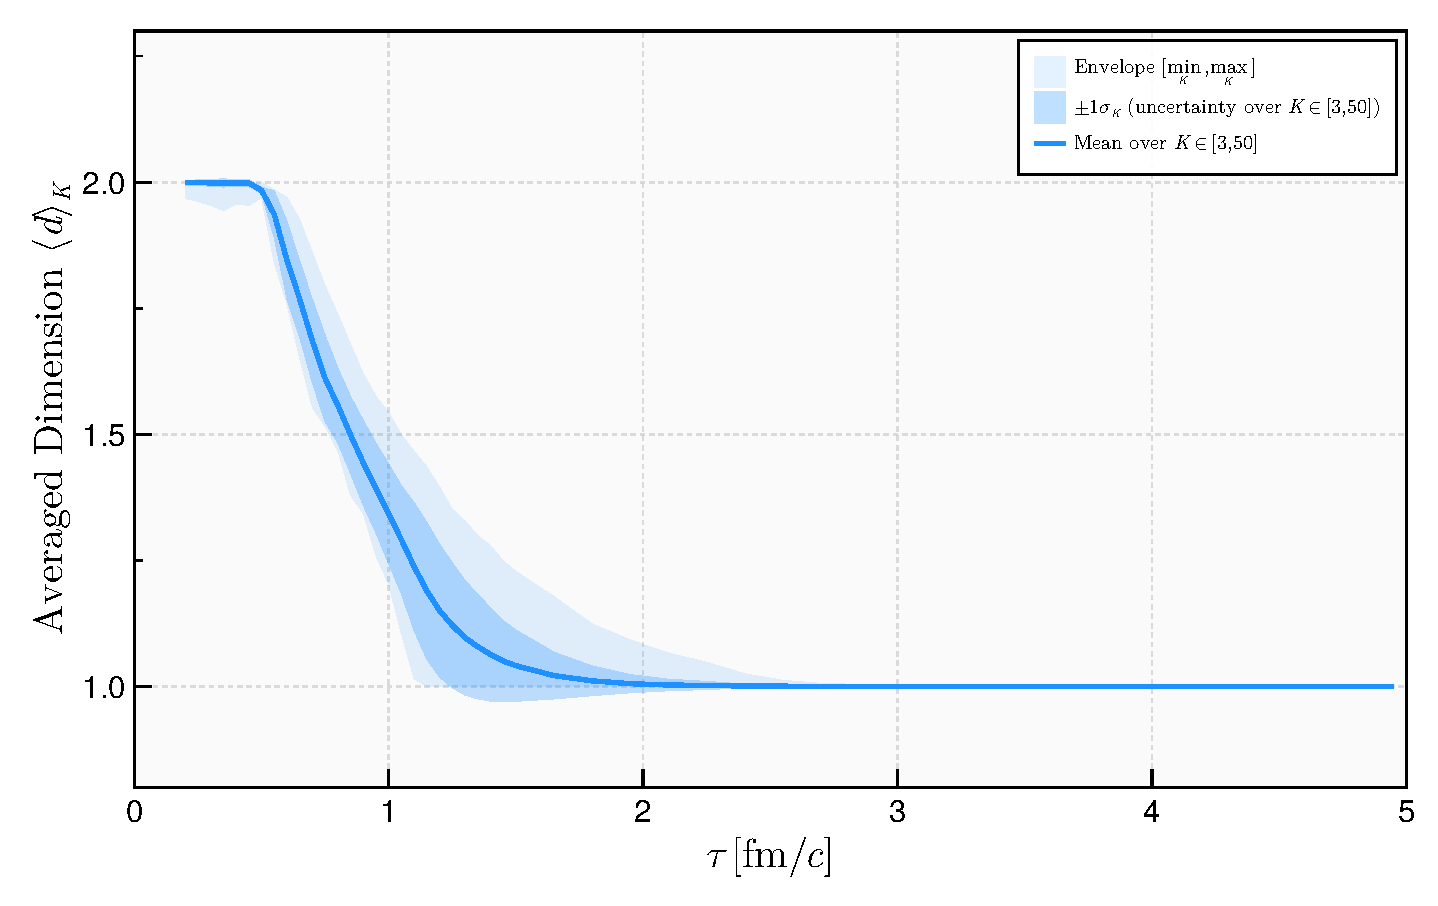
\includegraphics[width=\linewidth]{d_vs_tau_k_dependency/d_vs_tau_mis_zscore_k_averaged_dims.pdf}
        \caption{MIS: Średnia $\langle d \rangle_K$ (\emph{dims})}
        \label{fig:d_tau_mis_avg_dims}
    \end{subfigure}
    \hfill
    \begin{subfigure}[b]{0.48\textwidth}
        \centering
        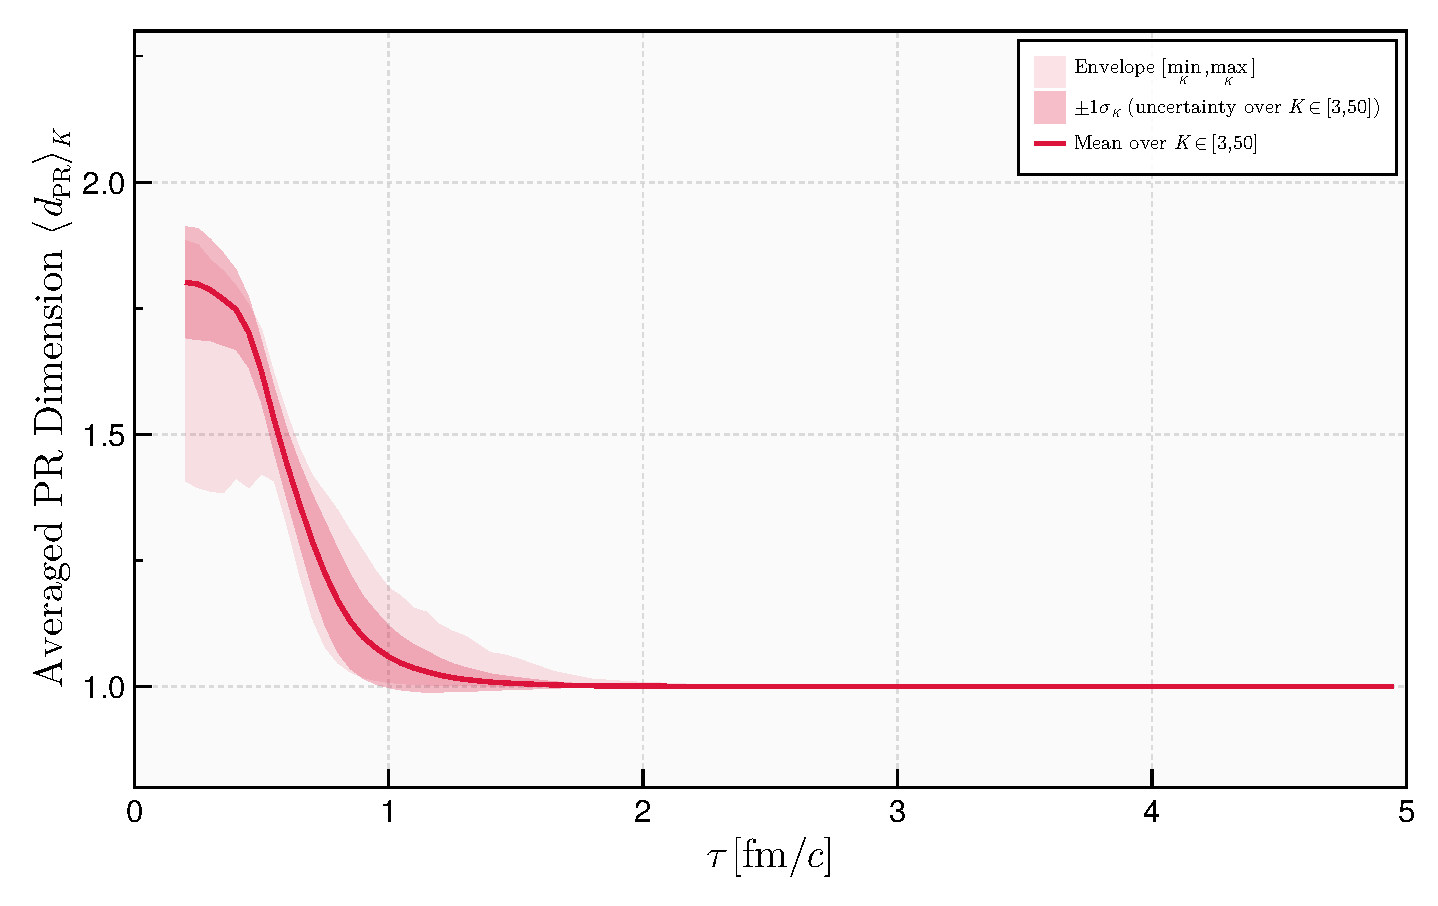
\includegraphics[width=\linewidth]{d_vs_tau_k_dependency/d_vs_tau_mis_zscore_k_averaged_pr.pdf}
        \caption{MIS: Średnia $\langle d_{\mathrm{PR}} \rangle_K$ (\emph{pr})}
        \label{fig:d_tau_mis_avg_pr}
    \end{subfigure}

    \vspace{0.8em}

    \begin{subfigure}[b]{0.48\textwidth}
        \centering
        \includegraphics[width=\linewidth]{d_vs_tau_k_dependency/d_vs_tau_hjsw_zscore_k_averaged_dims.pdf}
        \caption{HJSW: Średnia $\langle d \rangle_K$ (\emph{dims})}
        \label{fig:d_tau_hjsw_avg_dims}
    \end{subfigure}
    \hfill
    \begin{subfigure}[b]{0.48\textwidth}
        \centering
        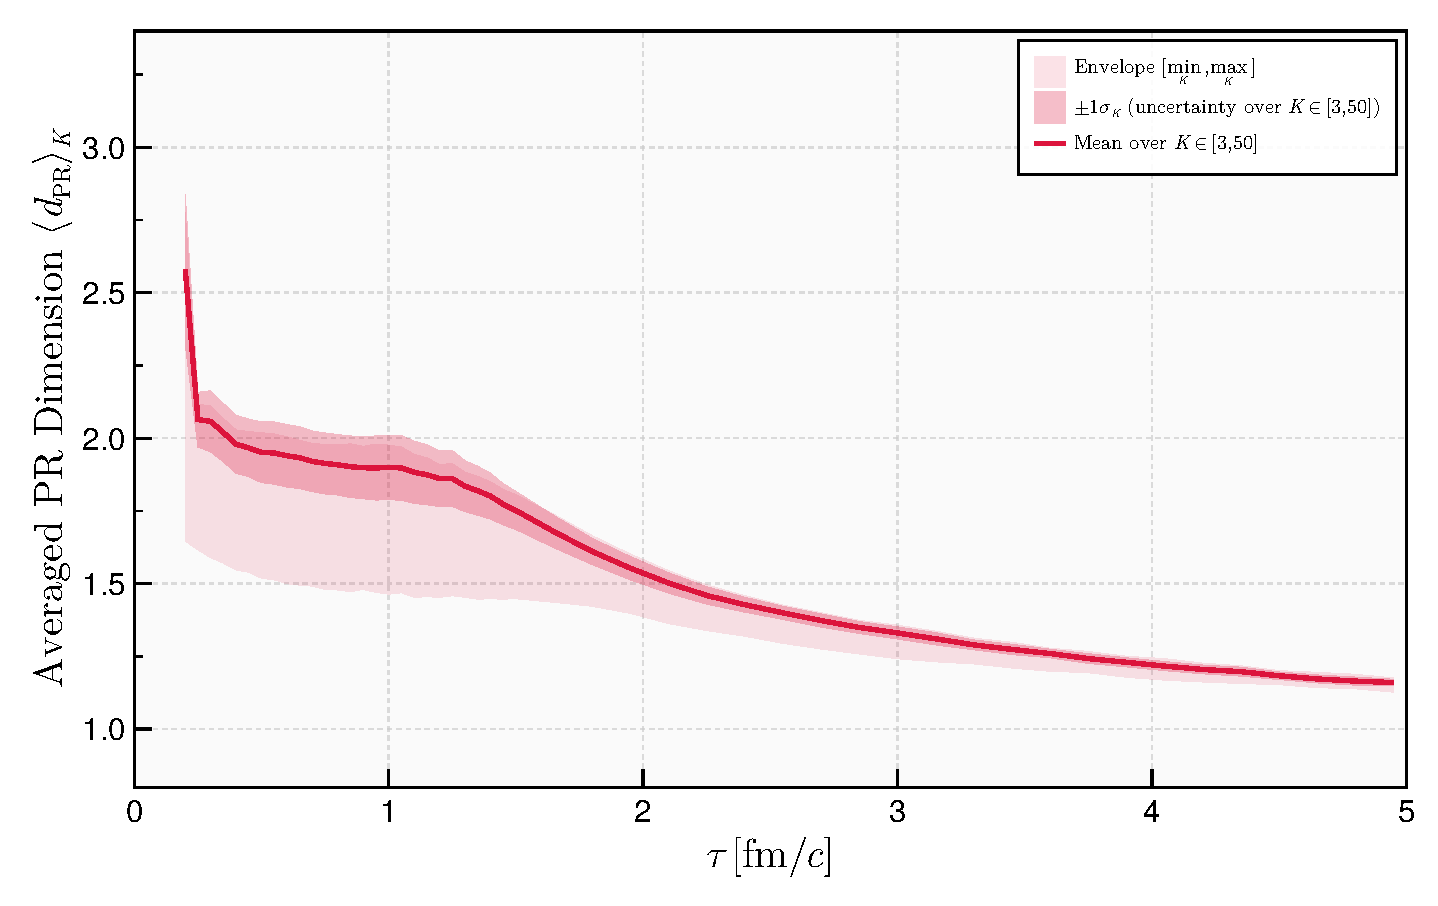
\includegraphics[width=\linewidth]{d_vs_tau_k_dependency/d_vs_tau_hjsw_zscore_k_averaged_pr.pdf}
        \caption{HJSW: Średnia $\langle d_{\mathrm{PR}} \rangle_K$ (\emph{pr})}
        \label{fig:d_tau_hjsw_avg_pr}
    \end{subfigure}

    \caption{Ewolucja wymiaru uśredniona po $K \in [3, 50]$. Ciemniejsze pasmo reprezentuje niepewność arbitralnego wyboru skali sąsiadów $\pm 1\sigma_K$, a jaśniejsze obwiednię $[\min_K, \max_K]$.}
    \label{fig:d_vs_tau_k_averaged}
\end{figure}
